\chapter{Introduction}

\section{Motivation}
Currently, rental room listings are posted on various sources such as real estate websites or Facebook groups. This makes the process of finding accommodations more challenging. Users often have to spend many hours on different websites to find a suitable room. Moreover, some sources for room listings lack the functionality to search according to users' needs. For example, in case of the rental posts on Facebook groups, users face a limitation in searching for posts based on crucial criteria such as price, location, or area,... Therefore, recognizing the problem, we want to build a system that centralizes all the rental posts in different sources and also provides an interactive way to search for posts based on users' preferences.

\section{Current solutions}
In this section, we will discuss some related works that are relevant to our thesis and represent the advantages and disadvantages of them.

\subsection{Facebook pages and groups}
Facebook is the most popular social network in the work. Therefore, Facebook pages and groups also become popular platforms for people to post their rental listings, as well as find accommodations. With the keyword "phòng trọ" you can see there are a lot of groups/pages with more than 100.000 members and >10 posts per day in Figure \ref{fig:facebook-group}

\begin{figure}[ht]
    \centering
    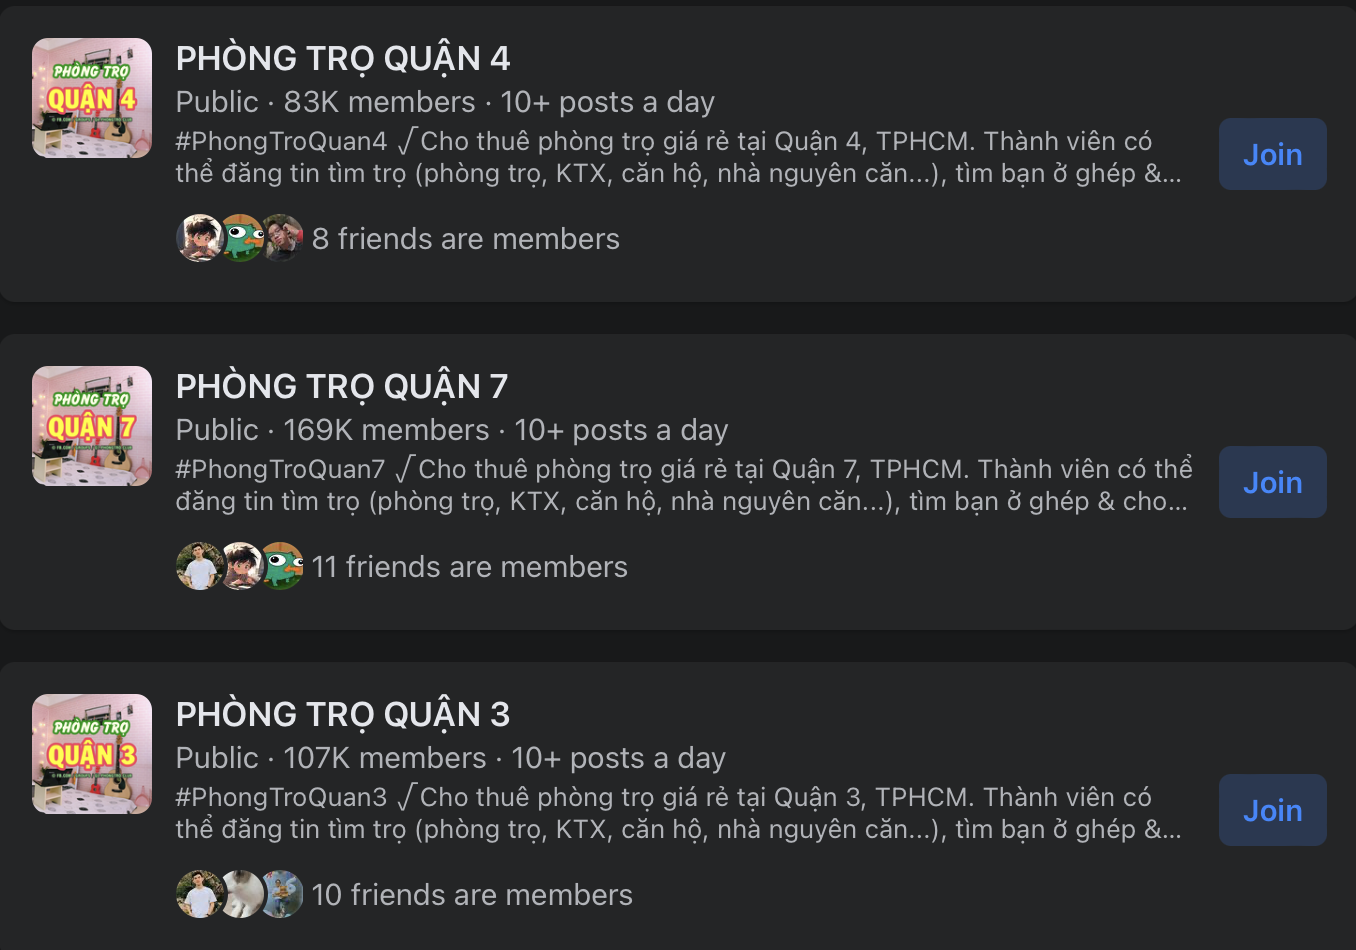
\includegraphics[width=0.8\textwidth]{images/1.Introduction/facebook_groups.png}
    \caption{The list of Facebook groups with the keyword "phòng trọ"}
    \label{fig:facebook-group}
\end{figure}

\noindent So Facebook is a good source for users to find accommodations. However, there are some disadvantages when using Facebook to find accommodations:
\begin{itemize}
    \item \textbf{The data is distributed in groups/pages}: There are many groups/pages for rental listings on Facebook. Therefore, users have to spend a lot of time with each group and find suitable accommodations.
    \item \textbf{Lack of search functionality}: Facebook does not provide a search functionality for users to search for posts based on their preferences. Therefore, users have to scroll through the posts to find the suitable ones.
\end{itemize}

\subsection{Real estate websites}
In the real estate market, many websites provide rental listings. Some of the most popular websites are nhattot.vn, batdongsan.com.vn, mogi.vn,... These websites provide a search functionality for users to search for rental listings based on their preferences. However, these websites do not have much data compared to Facebook groups/pages. Therefore, users have fewer choices when using these websites. One reason for that is the process of posting a rental listing on these websites is more complicated than on Facebook. Moreover, these websites provide different interfaces for users to interact with. Therefore, users have to get used to the user interface of each website. This makes the process of finding accommodations more challenging.

\section{Goal}
Understanding the problem of current websites in the market, we aim to provide a new solution that helps users find accommodations more easily. Our goal is to build an application that collects rental data from both Facebook groups/pages and real estate websites and provides a unified user interface. So instead of jumping between different websites, users can use our application to search for rental posts from different sources in one place. Moreover, our system also provides a chatbot interface to help users search for rental posts based on their preferences naturally and interactively. The feature list is shown below
\begin{itemize}
    \item Develop a crawler to collect rental data from Facebook groups, pages and other popular websites for finding accommodations in Vietnam such as nhattot.vn, batdongsan.com.vn.
    \item The data crawled from Facebook groups and pages is in the unstructured format. Therefore, we need to develop a Machine Reading comprehension model to extract the structured data from the unstructured data.
    \item Develop a website to display rental posts and allow the landlords to post their rooms for rent.
    \item Build the conversational chatbot that supports searching for rental posts based on users' preferences.
\end{itemize}

\section{Scope}
In the scope of this project, we mainly focus on the following tasks:

\begin{itemize}
    \item \textbf{Crawler}: we develop a crawler first, to collect the data from different sources. The data is also used to train the Machine Reading comprehension model.
    \item \textbf{Intent classification}: we build a modal to classify the user's intent based on the user's message.
    \item \textbf{Named Entity Recognition}: we build a model to extract the entities from both the user's message and the rental posts on Facebook pages. We want to get the structured data from the unstructured text.
    \item \textbf{Rental Website}: a website allows landlords to post their room for rent and users to search for accommodations.
    \item \textbf{Chatbot}: we built a chatbot to help users search for rental posts based on their preferences.
\end{itemize}
